%% =====================================================================
%%  GRAPHICAL ABSTRACT -- Confidence-Guided Adaptive Reconstruction
%%
%%  Generated from Figure 1 of A_method.tex. Do not edit by hand; edit the
%%  schematic in A_method.tex and regenerate.
%%
%%  Build:
%%    pdflatex graphical_abstract
%%    pdftocairo -png -r 300 -singlefile graphical_abstract.pdf graphical_abstract
%%
%%  Elsevier requires at least 1328 x 531 px at 300 dpi.
%% =====================================================================
\documentclass[border=6pt]{standalone}

\usepackage{amsmath,amssymb}
\usepackage{tikz}
\usetikzlibrary{arrows.meta,positioning,fit,backgrounds}

\newcommand{\Cw}{C_w}
\newcommand{\dcov}{\delta_{\mathrm{cov}}}
\newcommand{\Smax}{S_{\max}}
\newcommand{\beammax}{\texttt{beam\_max}}

\begin{document}
\begin{minipage}{20cm}
\centering
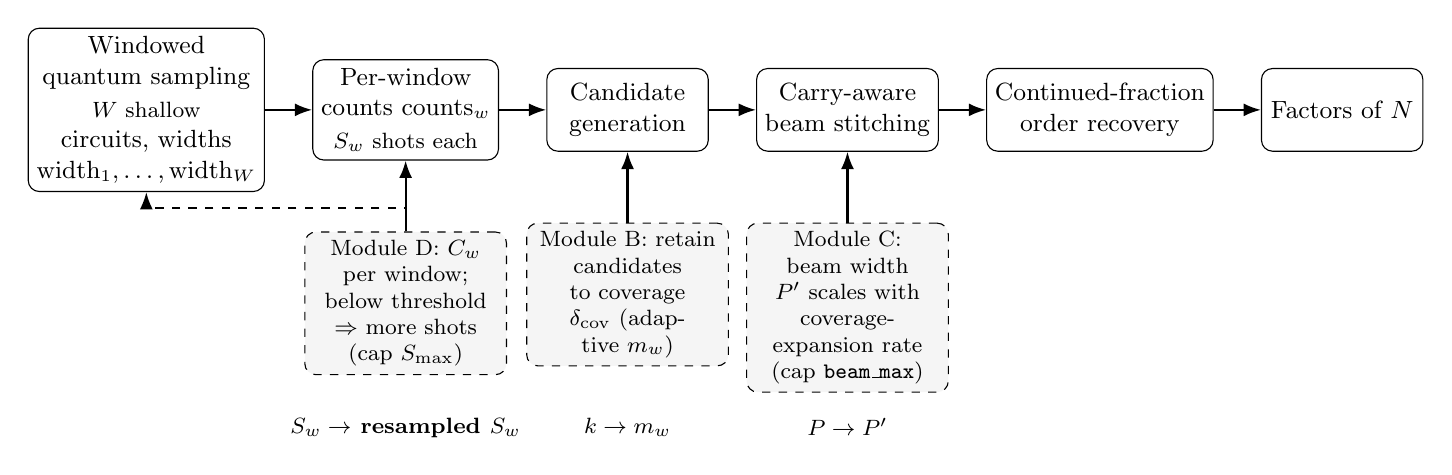
\begin{tikzpicture}[
  font=\small,
  box/.style={draw, rounded corners, align=center, minimum height=1.05cm, minimum width=2.05cm, inner sep=3pt},
  mod/.style={draw, dashed, rounded corners, align=center, minimum height=0.85cm, fill=gray!8, inner sep=3pt,
            text width=2.35cm, font=\footnotesize},
  arr/.style={-{Latex[length=2.2mm]}, thick},
  node distance=6mm
]

\node[box] (sample) {Windowed\\quantum sampling\\[1pt]\footnotesize $W$ shallow\\circuits, widths\\$\mathrm{width}_1,\dots,\mathrm{width}_W$};
\node[box, right=of sample] (counts) {Per-window\\counts $\mathrm{counts}_w$\\[1pt]\footnotesize $S_w$ shots each};
\node[box, right=of counts] (candgen) {Candidate\\generation};
\node[box, right=of candgen] (stitch) {Carry-aware\\beam stitching};
\node[box, right=of stitch] (order) {Continued-fraction\\order recovery};
\node[box, right=of order] (factors) {Factors of $N$};

\draw[arr] (sample) -- (counts);
\draw[arr] (counts) -- (candgen);
\draw[arr] (candgen) -- (stitch);
\draw[arr] (stitch) -- (order);
\draw[arr] (order) -- (factors);

\node[mod, below=9mm of counts] (moduleD) {Module D: $\Cw$ per window;\\below threshold $\Rightarrow$ more shots\\(cap $\Smax$)};
\node[mod, below=9mm of candgen] (moduleB) {Module B: retain\\candidates to coverage\\$\dcov$ (adaptive $m_w$)};
\node[mod, below=9mm of stitch] (moduleC) {Module C: beam width\\$P'$ scales with\\coverage-expansion rate\\(cap $\beammax$)};

\draw[arr] (moduleD) -- (counts);
\draw[arr, dashed] (moduleD.north) -- ++(0,3mm) -| (sample.south);
\draw[arr] (moduleB) -- (candgen);
\draw[arr] (moduleC) -- (stitch);


\path (moduleC.south) ++(0,-2mm) coordinate (annobase);
\node[font=\footnotesize\bfseries, anchor=north] at (moduleD |- annobase) {$S_w \to$ resampled $S_w$};
\node[font=\footnotesize\bfseries, anchor=north] at (moduleB |- annobase) {$k \to m_w$};
\node[font=\footnotesize\bfseries, anchor=north] at (moduleC |- annobase) {$P \to P'$};
\end{tikzpicture}

\vspace{3mm}
\hrule
\vspace{2mm}

{\footnotesize
Fixed top-$k$ retention captures \textbf{0.571} of the true per-window
probability mass; coverage-based retention captures \textbf{0.841}, and does
so almost independently of how $k$ was set. The quantum circuit is unchanged.
\par}
\end{minipage}
\end{document}
